\subsection{Milestones}
Our team has decided to utilize the Agile approach for this project. We chose this methodology because it allows our team to focus on sections of the project and aligns well with the semester schedule. By making iterations for this project internally, we are able to track our progress and make status updates. Another benefit of this will be tracking any delays or problems. If we are behind on a section, we have already planned ahead and allowed ourselves room for some variance. We are also using smaller deliverables for the project which gives us more tracking because we have more internal deadlines. We will be using Jira to track our progress and add reports throughout the process. We will also be utilizing Discord as a form of communication with each other. This will be a place where we can discuss any issues or ask quick questions when we are not in person. Below, we have a high-level breakdown written for our project goals.
\subsubsection{Fall}
\begin{itemize}
        \item Document selection reasoning
        \item Order to ensure on-time delivery
        \item Model physical bed
\end{itemize}
\subsubsection{Spring}
\begin{itemize}
    \item Model physical bed
    \item Build physical bed
    \item Test subsystems in isolation
    \item Start integrating subsystems
    \item MCU coding complete
\end{itemize}

\subsection{Progress}
In the following two sections the team will discuss the progress made in each of the two semesters.
\subsubsection{Senior Design I}
Senior Design I was a culture shock for the team. Looking back at the eli\textsuperscript{2} training, the team took a long time to form, and almost the rest of the semester to storm, only to finally start norming and performing at the end of the semester. The team by November was ordering parts and waiting patiently on their arrival only to realize there was no method to how integrations would occur. The entire process seemed a little backwards. Moving forward, the team has found a way to hold each other accountable to the tasks that we are performing and hope to be more productive over the break and through the fall.
\begin{figure}[H]
    \caption{Cumulative Flow Diagram from Jira}
    \centering
    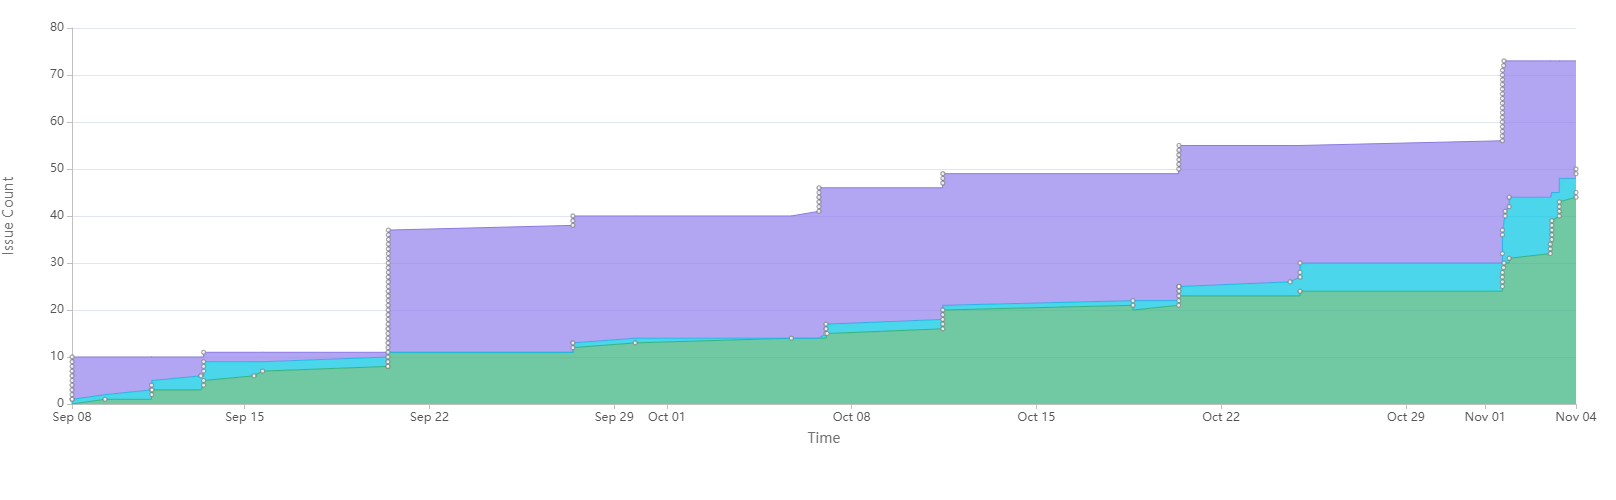
\includegraphics[width=\textwidth]{images/Cumulative flow diagram.png}
    \label{fig:cumulativeflow}
\end{figure}
In Figure \ref{fig:cumulativeflow}: purple designates tasks that are marked unfinished in the the backlog and current sprint, blue represents in progress tasks, and green represents finished tasks.

Throughout Senior Design I we have been gathering research and have started laying out the design of our garden bed and have completed the majority of our part selection. The Figure in \ref{fig:cumulativeflow} may be a little misleading at this point because we have not refined our backlog to fully encapsulate meaningful tasks instead breaking it down into larger subsystem requirement-esque tasks.

\subsubsection{Senior Design 2}
Over the break, the team took time to reset before the big grind semseter.
When we got back, the team met more frequently, 3 times a week to get a progress update. Below the cumulative flow diagram shows how the team buttoned down to accomplish a lot throughout the semester.
The big items that the team had to conquer were testing and having to iterate over all the designs several times.
For example, after breadboarding the sensing subsystem, the team decided to go ahead and order PCBs before coming to a realization the design would not work with the ADC.

\begin{figure}[H]
    \caption{Senior Design 2 Cumulative flow diagram}
    \centering
    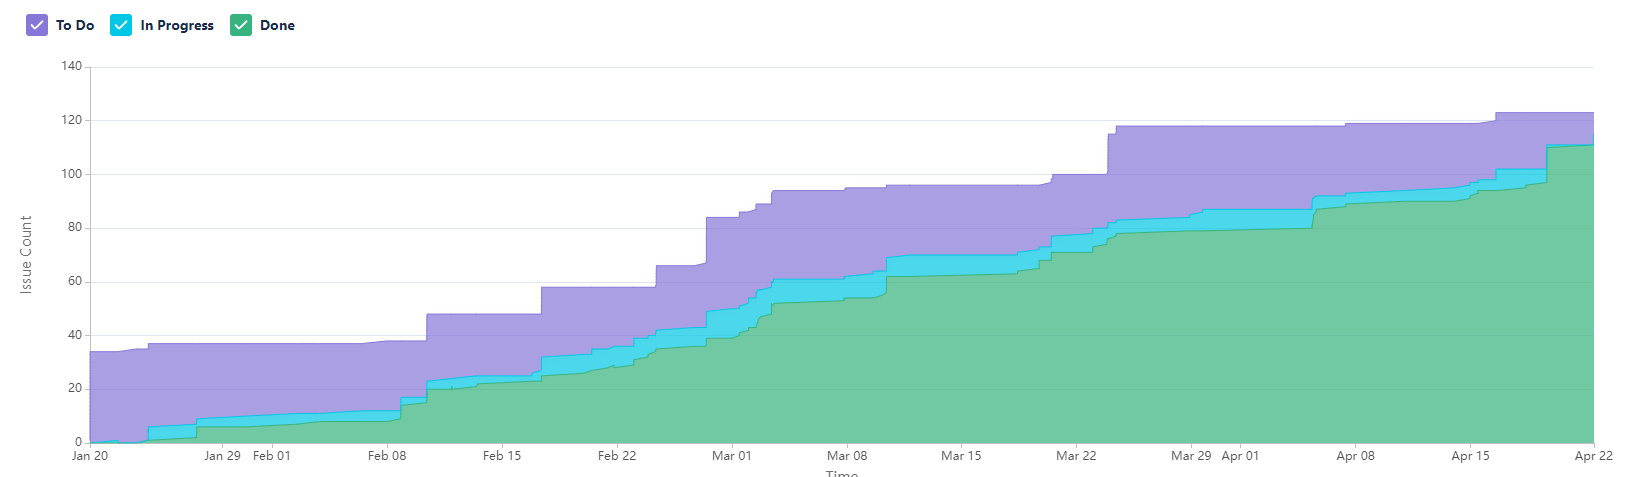
\includegraphics[width=\textwidth]{images/Cumulative flow diagram-sd2.PNG}
    \label{fig:cumulativeflow}
\end{figure}

From the diagram, there was much more consistent project by the team and some of that can be attributed to a greater level of organization through a greater dedication to Jira.